\chapter{ Description of the model \label{ch:numero_uno}}
\section{An invitation to Signed Distance Fields}
The use of signed distance fields (SDFs) to model organic sufaces is a time honoured graphical technique used, for example, by Pixar Animation Studios to model hair 
in \textit{The Incredibles} (see \cite{petrovic2005volumetric}). The idea is to define a function which represents the closest distance
from the query point to a point on the surface of the object that is to be represented. If the query point is outside, the SDF is positive,
 the SDF is zero on the surface and negative inside. SDFs can be rendered within traditional graphics pipelines (such as OpenGL or Vulkan) using raymarching, 
 a method that takes place within shader programs and is therefore meshless. The formulae defining SDFs for common 2D and 3D shapes are easy to find online, see
 \cite{key}. Whilst the simulations herein are done using 2D SDFs, a quick 3D primer is given below.
 
 To motivate the primary mechanism by which cells will undergo mitosis in this thesis, we consider a toy example in which the equations for two spheres undergo a catastrophic topological change as one parameter changes. 
 We start by considering the equations for two spheres which begin as coincident and move apart as the parameter $a$ becomes larger. In order to combine the first equation
\begin{equation*}
f_1(x,y,z) =  \sqrt{ (x+a)^2+y^2+z^2 } -R,
\end{equation*}
with the second equation
\begin{equation*}
f_2(x,y,z) =  \sqrt{(x-a)^2+y^2+z^2 } - R,
\end{equation*}
we require a smooth combination function. We construct the combined SDF using what is called a ``union" in the graphics community (see \cite{fusekvisualization}).
This is the pointwise minimum 
\begin{equation*}
f_{\textrm{union}}(x,y,z) = \min(f_1(x,y,z), f_2(x,y,z)).   % \frac{1}{k}\ln{ \left( e^{k f_1(x,y,z)}+ e^{k f_2(x,y,z)} \right) }.
\end{equation*}
In reality, it may be nicer to have a smooth transition between the cells at a given point of time. That is why we use 
$\textrm{smoothmin}$ which is defined by a smoothness parameter $k$, as in
\begin{equation}
    \textrm{smoothmin}(x_1, x_2) = -k \log(e^{-x_1/k} + e^{-x_2/k}).
\end{equation}
As shown in Figure \ref{fig:ToyMitosis}, we have a smooth splitting of a cell as the parameter $a$ ranges from $0.0$ to $5.0$.
Note that $R$ is the nominal sphere radii, and $k$ is a smoothing parameter. The larger $k$ is, the more smoothly the two curves cling to each other. 
We plot the level-$0$ surface of the smooth union SDF using MATLAB's \codeword{isosurface} function. 

\begin{figure}[h]
\centering
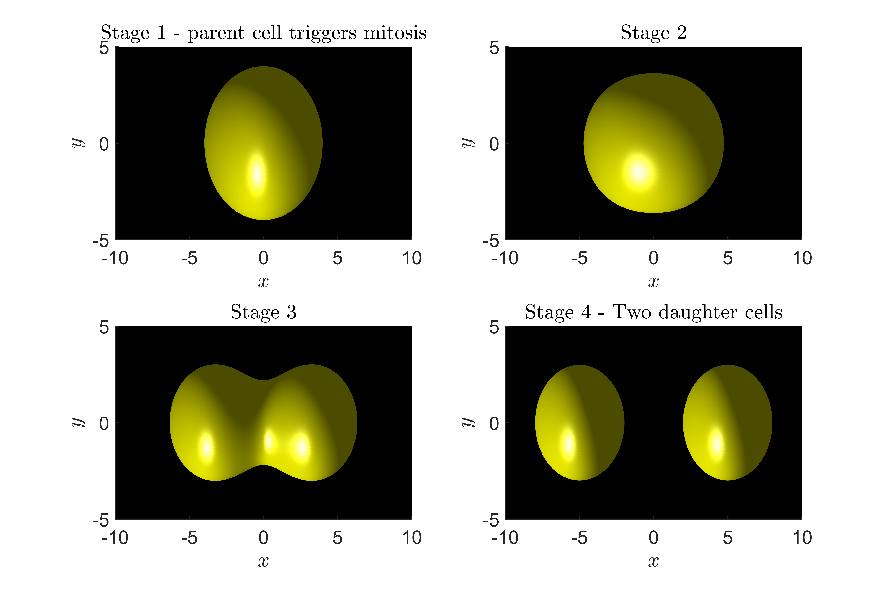
\includegraphics[width=1\textwidth]{chapter1/figures/CellDivisionDemo.pdf}
\caption{A toy example of mitosis using implicit equations for spheres in 3D. Stage 1 is $a= 0.0$, Stage 2 is $a= 1.67$, Stage 3 is $a=3.33$, Stage 4 is $a = 5.0$}
\label{fig:ToyMitosis}
\end{figure}
\filbreak

It is also possible to get the intersection of two SDFs using a $\textrm{smoothmax}$ function.

\section{Modeling growing geometry }
Cell colonies can be built up by combining the SDFs of the individual cells using a cumulative $\textrm{smoothmin}$. We employ
the main aspect of $\textrm{smoothmin}$, which is that 
\begin{equation}
    \textrm{smoothmin}(f_3, \textrm{smoothmin}(f_1,f_2)) = -k \log( \sum_{j=1}^3 e^{-f_j/k}),
\end{equation}
therefore we can accumulate smoothmins easily using
\begin{equation}
    \textrm{smoothmin}(f_1, \ldots, f_N) = -k \log( \sum_{j=1}^N e^{-f_j/k}),
\end{equation}

The individual cells are modelled using the approximate signed distance field for an ellipse which is given at 
\url{https://www.shadertoy.com/view/4XfBDl}. I have provided the vectorized MATLAB implementation below,

\begin{lstlisting}[style=Matlab-editor]
    function sdf = ellisoid_sdf(x, y, theta, r, X, Y)
        semi_minor_axis = min(r);
        semi_major_axis = max(r);
        c = sqrt(semi_major_axis^2 - semi_minor_axis^2);
        %Geometrical parameter
        center = [x,y]';
        query_point = [X(:), Y(:)]';
        R_z = rotation_matrix(theta);
        l1 = vecnorm(pagemtimes(R_z , query_point - center) - [c;0], 2, 1);
        l2 = vecnorm(pagemtimes(R_z , query_point - center) + [c;0], 2, 1);
        l = mean([l1', l2'],2);
        sdf = reshape(l', size(X)) - semi_major_axis;
    end 
\end{lstlisting}
Note that I multiply each local coordinate \codeword{query_point - center} by the rotation matrix \codeword{R_z} in order
to rotate the cell counter-clockwise by $\theta$ radians. The rotation matrix $R_z$ is given by
\begin{equation}
    R_z = \begin{bmatrix}
            \cos{(\theta)} & \sin{(\theta)}\\
            -\sin{(\theta)} & \cos{(\theta)} 
        \end{bmatrix} ,
\end{equation}
which is a so-called passive rotation matrix because we are rotating the coordinate system by $\theta$ CW which has the effect 
of rotating the ellipse by $\theta$ CCW.


\section{Cell-cell collisions with constrained dynamics}
Earlier, it was mentioned that the intersection of cells could be found by taking a smoothmax. To find the overlapping area
the sum of the grid points in the intersection can be taken and then multiplied by the grid square area $h_x h_y$. Whilst
it is more or less trivial to calculate the overlapping area, ensuring that this area remains zero throughout the simulation
is more involved. We employ the technique explained by \cite{witkin1997introduction} based on constrained
dynamics. The constraint in this case is that the area $C$ remains $0$ for all times,
\begin{equation}
    C(\vb{q}) = 0,
\end{equation}
where $\vb{q}$ is the concatenated state vector of the system. One should be aware that, if we have multiple colonies, it will
be required to have pairwise constraints forcing no overlap between each of the constitiuent colonies. For the purpose of simplicity
our state vector $\vb{q}$ will just take into account position and orientation and not size of cells. Later on, this will be generalized.
Therefore $\vb{q}$ is produced by concatenating over $\vb{q}_j$ into one $3N \times 1$ column vector, where
\begin{equation}
\vb{q}_j = \begin{bmatrix}
                x_j \\
                y_j \\
                \theta_j
            \end{bmatrix}.
\end{equation}
Of course, the number of variables per cell can be larger but this comes at a cost in computational time. Recall that the 
intersecting area is secretly a function of the cell state coordinates $\vb{q}_j$ since we are taking a smoothmax of the SDFs 
of each cell. In other words,
\begin{equation*}
f_{\textrm{intersect}}(x,y,\vb{q}) = \textrm{smoothmax}(f_1(x,y,\vb{q}) , \ldots, f_N(x,y,\vb{q}) ),
\end{equation*}

for concreteness, we write out the formula for smoothmax which is the negative smoothmin of the negatives of the SDFs or
\begin{equation*}
    f_{\textrm{intersect}}(x,y,\vb{q}) = -\textrm{smoothmin}(-f_1(x,y,\vb{q}) , \ldots, -f_N(x,y,\vb{q}) ).
\end{equation*}
In full this boils down to,
\begin{equation*}
    f_{\textrm{intersect}}(x,y,\vb{q}) = k \log( \sum_{j=1}^N e^{f_j(x,y,\vb{q})/k}).
\end{equation*}
Now we assume the state is given by five variables for full generality:
\begin{equation}
\vb{q}_j(t) = 
\begin{bmatrix}
    x_j (t) \\
    y_j(t) \\
    \theta_j(t) \\
    b_j(t) \\
    R_j(t)
\end{bmatrix},
\end{equation}
where $b(t)$ is the semi-major axis length and $R_j(t) \in (0,1]$ is the aspect ratio of the elliptical cell so the semi-minor axis is given by $a_j(t) = R_j(t) b_j(t)$. 
Why are we going to the effort to write out $C(\vb{q})$ in full? Because we need to compute the Jacobian of $C(\vb{q})$ with
respect to $\vb{q}$ in order to carry out the constrained dynamics algorithm. The upshot is that smoothmax is differentiable
whereas maximum is not differentiable. 

We define the region in $\mathbb{R}^2$ to integrate over by 
\begin{equation}
    \Omega(\vb{q}) = \{ (x,y) \in \mathbb{R}^2 \ | \ f_{\textrm{intersect}}(x,y,\vb{q}) \leq 0 \},
\end{equation}
so that the area of the overlapping region is simply a two-dimensional integral over $\Omega(\vb{q})$ of $1$,
\begin{equation}
    C(\vb{q}) = \int\int_{\Omega(\vb{q})} dxdy.
\end{equation}
Now we break up the integral into a sum over simply connected components (SCC) so that we can safely apply Leibniz's rule
\begin{equation}
    C(\vb{q}) = \sum_{i \in SCC(\vb{q})}\int\int_{\Omega_i(\vb{q})} dxdy.
\end{equation}
Leibniz's rule tells us how to carry out a total derivative of $\int\int_{\Omega_i(\vb{q})} dxdy$ with respect to $t$ which determines $\vb{q}$. Let's take that total
derivative now to attain
\begin{equation}
   \frac{d}{dt}\int\int_{\Omega_i(\vb{q})} dxdy = \int\int_{\Omega_i(\vb{q})} \pdv{(1)}{t} dxdy + 
   \int_{\partial \Omega_i(\vb{q})} (1) \vb{v}_{\partial \Omega_i(\vb{q})} \cdot \hat{\vb{n}} dl,
\end{equation}
where $\vb{v}_{\partial \Omega_i(\vb{q})}$ is the ``Eulerian'' velocity of the boundary of the $i$-th SCC. All of this can be avoided if we integrate over a smoothstep
which is defined in our region.
\begin{equation}
    C(\vb{q}) = \int\int_{D} \left[ \frac{1}{2} +\frac{1}{2} \tanh{ \left(- \frac{1}{K}f_{\textrm{intersect}}(x,y,\vb{q}) \right)}\right]dxdy,
\end{equation}
where $D$ is the entire domain of the pertri dish.


\begin{equation*}\
\pdv{f_{\textrm{intersect}}(x,y,\vb{q})}{\vb{q}} = \frac{ \sum_{j=1}^N \pdv{f_j(x,y,\vb{q})}{\vb{q}}e^{f_j(x,y,\vb{q})/k}}{ \sum_{j=1}^N e^{f_j(x,y,\vb{q})/k}}.
\end{equation*}
Conveniently, computing the Jacobian, has turned into $N$ problems that are easier to solve individually. Namely computing $\pdv{f_j(\vb{q})}{\vb{q}}$.
This requires us to express the SDF for an ellipse in terms of the query point $(x,y)$, the center of the cell $(x_j,y_j)$, and its orientation $\theta_j$. This
is given in terms of $l_j^-(\vb{q}, x, y)$ and $l_j^+(\vb{q}, x, y)$ which are given in the ellipse formula. We use MATLAB's symbolic toolbox to compute the
ellipse Jacobian $\pdv{f_j(x,y,\vb{q})}{\vb{q}}$ and return a function that can take numerical inputs using \codeword{matlabFunction(J,"File","ellipseJacobian")}.
With that we can compute Jacobian of the constraint using
\begin{equation} 
    \pdv{C(\vb{q})}{\vb{q}} = -\frac{1}{2K} \int \int_D \left[ 1- \tanh[2]( -\frac{f_{\textrm{intersect}}(x,y,\vb{q})}{K}) \right] \pdv{f_{\textrm{intersect}}(x,y,\vb{q})}{\vb{q}} dx dy.
\end{equation}
Now that all the derivatives have been computed analytically, we can carry out the computation of the integral over $x$ and $y$ using a numerical integral in MATLAB.
From now we use $f$ instead of $f_{\textrm{intersect}}$ for brevity, and we pass to index notation, instead expression the $\beta$-th component of $J$ as 
\begin{equation}
J_{\beta} = -\frac{1}{2K} \int \int_D \left[ 1- \tanh[2]( -\frac{f(x,y,\vb{q})}{K}) \right] \pdv{f(x,y,\vb{q})}{q_{\beta}} dx dy.
\end{equation}
For the computation of constraint forces, we need to further compute the total derivative of the Jacobian with respect to time. This turns 
out to be realted to the Hessian matrix of $C(\vb{q})$ (for no explicit time dependence), as 
\begin{equation*}
    \dot{J}_{\beta} = \sum_{\alpha = 1}^{5N} \dot{q}_{\alpha} \frac{\partial^2 C}{ \partial q_{\alpha} \partial q_{\beta}} = \sum_{\alpha = 1}^{5N} \dot{q}_{\alpha} H_{\alpha, \beta},
\end{equation*}
We need to compute how the Hessian of $C$ can be written in terms of the Hessian and Jacobian of $f$.
\begin{equation}
    \frac{\partial^2 C}{ \partial q_{\alpha} \partial q_{\beta}} = \frac{\partial }{\partial q_{\alpha}} J_{\beta}
\end{equation}
Crunching the calculuations we get
\begin{equation}
 \frac{\partial }{\partial q_{\alpha}} J_{\beta} = -\frac{1}{4 K^2} \int \int_D \left[ 1- \tanh[2]( -\frac{f}{K}) \right] \left[\tanh(-\frac{f}{K})\pdv{f}{q_{\alpha}}\pdv{f}{q_{\beta}} + K \frac{\partial^2 f}{ \partial q_{\alpha} \partial q_{\beta}}\right]  dx dy
\end{equation}
Luckily, the Hessian is built into MATLAB's symbolic toolbox, so we can just call \codeword{matlabFunction(H,"File","ellipseHessian")} and the function to compute
the Hessian is saved into our working directory. Note that the function \codeword{ellipseHessian} computes a $5 \times 5 \times N_{\textrm{grid}} \times N_{\textrm{grid}}$ matrix. 
We call it for each cell $j \in \{1, \ldots, N\}$ but recall that for a given value of $\vb{q}$, the Hessian still has $(x,y)$ as free field variables. In order to integrate
the field data, we use the cell-wise Jacobian field $J_{\beta}^j (x,y)$ and the cell-wise Hessian field $H_{\alpha, \beta}^j (x,y)$ to calculate the overall Hessian field for $f$
\begin{equation*}
    \frac{\partial^2 f}{ \partial q_{\alpha} \partial q_{\beta}} = \left(\frac{1}{k}\right) \left[ \frac{\left(\sum_{j=1}^N E_j\right) \left( \sum_{j=1}^N E_j (k H_{\alpha, \beta}^j + J_{\alpha}^j J_{\beta}^j)\right) - \left(\sum_{j=1}^N E_j J_\alpha^j \right) \left(\sum_{j=1}^N E_j J_\beta^j \right)}{\left(\sum_{j=1}^N E_j\right)^2} \right],
\end{equation*}
where $E_j = e^{f_j/k}$ is used for short. To actually compute the overall integrals for $\pdv{C}{q_{\beta}}$ and $\frac{\partial^2 C}{ \partial q_\alpha \partial q_\beta }$
we use MATLAB's \codeword{trapz} function the following way
\begin{lstlisting}[style=Matlab-editor]
    trapz(y_lin,trapz(x_lin,integrandJacobian,3),2);
\end{lstlisting}
or, in the case of the Hessian,
\begin{lstlisting}[style=Matlab-editor]
    trapz(y_lin,trapz(x_lin,integrandHessian,4), 3);
\end{lstlisting}
where the integrand in the Jacobian cas is given by
\begin{equation*}
    F_{\beta}(x,y) = \left(\frac{T^2-1}{2K} \right)\frac{ \sum_{j=1}^N J_\beta^j E_j}{ \sum_{j=1}^N E_j},
\end{equation*}
where $T = \tanh( -\frac{f(x,y,\vb{q})}{K})$ and, in the case of the Hessian
\begin{equation*}
    G_{\alpha, \beta}(x,y) = 
\left(\frac{T^2-1}{4K^2} \right) \left(T \left(\frac{ \sum_{j=1}^N J_\alpha^j E_j}{ \sum_{j=1}^N E_j}\right) \left(\frac{ \sum_{j=1}^N J_\beta^j E_j}{ \sum_{j=1}^N E_j}\right) + K \frac{\partial^2 f}{ \partial q_{\alpha} \partial q_{\beta}} \right),
\end{equation*}
which, after some serious simplification becomes
\begin{equation*}
    G_{\alpha, \beta}(x,y) = \frac{T^2-1}{4Kk \left(\sum_{j=1}^N E_j\right)^2} \sum_{n=1}^N \sum_{m=1}^N E_n E_m \bigg[ \left( \frac{kT-K}{K}\right) J_\alpha^n J_\beta^m +J_\alpha^m J_\beta^m +k H_{\alpha, \beta}^m \bigg]
\end{equation*}
To make things neat we replace $B = \frac{T^2-1}{4K^2}$, $\hat{E} = \sum_{j=1}^N E_j$ and we subsitute the ratio of the smoothstep and smoothmax parameters
$S = K/k$ to attain,
\begin{equation*}
    G_{\alpha, \beta}(x,y) = \frac{B}{\hat{E}^2} \sum_{n=1}^N \sum_{m=1}^N E_n E_m \bigg[   S(k H_{\alpha, \beta}^m +J_\alpha^m J_\beta^m )+ (T-S)J_\alpha^n J_\beta^m\bigg],
\end{equation*}
Thus we can write 
\begin{equation*}
    J_\beta =  \int \int_D F_{\beta}(x,y) dx dy,
\end{equation*}
\begin{equation*}
    \dot{J}_\beta =\sum_{\alpha=1}^{5N}\dot{q}_\alpha \int \int_D G_{\alpha, \beta}(x,y) dx dy,
\end{equation*}
Now we subsitute to obtain the final integral formulae:
\begin{equation*}
    J_\beta =  \int \int_D \frac{B}{\hat{E}S} \sum_{j=1}^N J_\beta^j E_j dx dy,
\end{equation*}
\begin{equation*}
    \dot{J}_\beta = \int \int_D \frac{B}{\hat{E}^2}  \sum_{\alpha=1}^{5N}  \sum_{n=1}^N \sum_{m=1}^N \dot{q}_\alpha E_n E_m \bigg[   S(k H_{\alpha, \beta}^m +J_\alpha^m J_\beta^m )+ (T-S)J_\alpha^n J_\beta^m\bigg] dx dy.
\end{equation*}
We set out to calculate the following scalar $A = JWJ^t$ where $W = M^{-1}$ is the inverse mass matrix of our dynmical system. Note, that since we have 
only one constraint our goal is to solve for one Lagrange multiplier $\lambda$ which is given as 
\begin{equation*}
A \lambda = - \sum_{\beta =1 }^{5N }\dot{J}_\beta \dot{q}_\beta - JWQ -k_s C -k_d \dot{C},
\end{equation*}

where $R$ is the radius of the circle. If the filled in circle, the disk, is required, then producing a surf plot of the function in the region where $f(x,y) \geq 0$ is sufficient. This can be achieved by modifying the value of $f(x,y)$ to be \codeword{nan} wherever $f(x,y)<0$ so that MATLAB's \codeword{surf} function does not plot it.
\\
\\
For approximately circular cells, each individual cell is modeled via the equation of a circle centered at position $(x_j(t),y_j(t))$ where $j$ indexes over the current total number of cells. The equation for a single cell is therefore given by
\begin{equation*}
    f_j(x,y;t) =R_j^2- \left[ (x-x_j(t))^2 + (y-y_j(t))^2\right],
\end{equation*}
where $R_j$ is the radius of the $j$-th cell. We will discuss how multiple cells can be blended together into one colony level implicit curve. Given the implicit curve for cell $1$ to cell $N = N(t)$, respectively $f_1(x,y;t), \cdots, f_N(x,y; t)$, we blend them with the following transformation
\begin{equation*}
    \tilde{\Phi}(x,y;t) = \frac{1}{k}\ln{ \left[ \frac{1}{N} \sum_{j=1}^N{ e^{k f_j(x,y;t)}} \right]},
\end{equation*}
where $\tilde{\Phi}(x,y;t) $ is related to the colony microscopic density, $k$ is a 
parameter related to the level of smoothing between the curves, $N$ is the total number of cells. 
If all of the $f_j(x,y;t) =0$ then we recover that $\tilde{\Phi}(x,y;t) =0$. Of course, we don't yet have the actual colony microscopic density, because the numerical values taken by $\tilde{\Phi}(x,y;t) $ are essentially meaningless. The microscopic density $\Phi(x,y;t)$ is obtained by translating and scaling $\tilde{\Phi}(x,y;t) $ such that $\Phi(x,y;t) $ takes values on the interval $[0,1]$. We then interpret $1$ as the maximum biomass density of the cell at each cell center.

\section{Mitosis: new cells from old}
The addition of new cells can be easily achieved by incorporating additional implicit curves and, hence, modifying the colony microscopic density $\Phi(x,y;t) $. In the case of circular cells which undergo effectively symmetric mitosis, it is necessary to add a cells at a slight offset so that contact forces (explained in the following section) can take effect. In order to store the data associated with each cell, a final number of cells $N_f$ is designated as a constant maximum number of cells which allows for the preallocation of the data associated with the cell centers and other state information (if necessary). 
\\
\\
One of the desired features of the model, was to achieve cell division (which can be thought of as a catastrophic change in the colony topology)  without sacrificing the smoothness of $\Phi(x,y;t) $. This has been achieved by starting the new cell at a vanishingly close distance to its parent cell, and recovering smoothness through the blending of implicit curves imposed in the construction of $\Phi(x,y;t)$. This is possibly a new idea in the field of agent based models, where the addition of daughter cells is usually not even continuous (for example, in some off-lattice ABMs new cells simply appear beside old ones). Here, the two daughter cells move apart via contact forces between the cell centers and the smooth division follows.

\section{Modeling interactions between cells}
In standard particle dynamic simulations, say gravitational models, the particle positions are modeled using Newton's second law. This means the state of an $N$ particle simulation in $2D$ requires $2N$ positions and $2N$ velocity values. In overdamped, low-inertia regime, which is often used in cell off-lattice ABMs, it is sufficient to ignore changes in the velocity and only construct equations for the change in position over time. 

\section{Tuning the model parameters}

\begin{figure}[h]
\centering
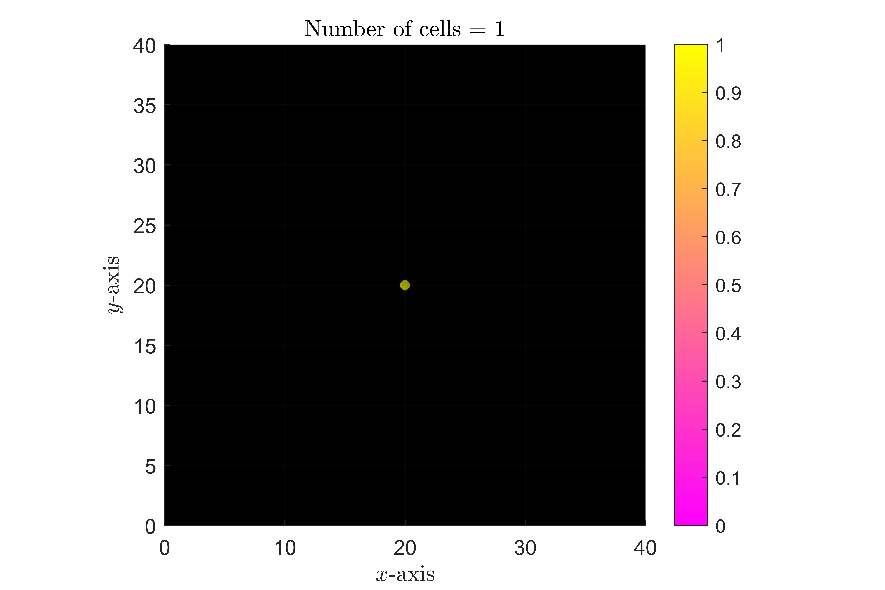
\includegraphics[width=1\textwidth]{chapter1/figures/ColonySimulationDemo_N_1.pdf}
\caption{A starting configuration consisting of a cell with radius $1$ unit equals $3.5 \mu m$}
\label{fig:ColonySimulationStartingCell}
\end{figure}
\filbreak


\begin{figure}[h]
\centering
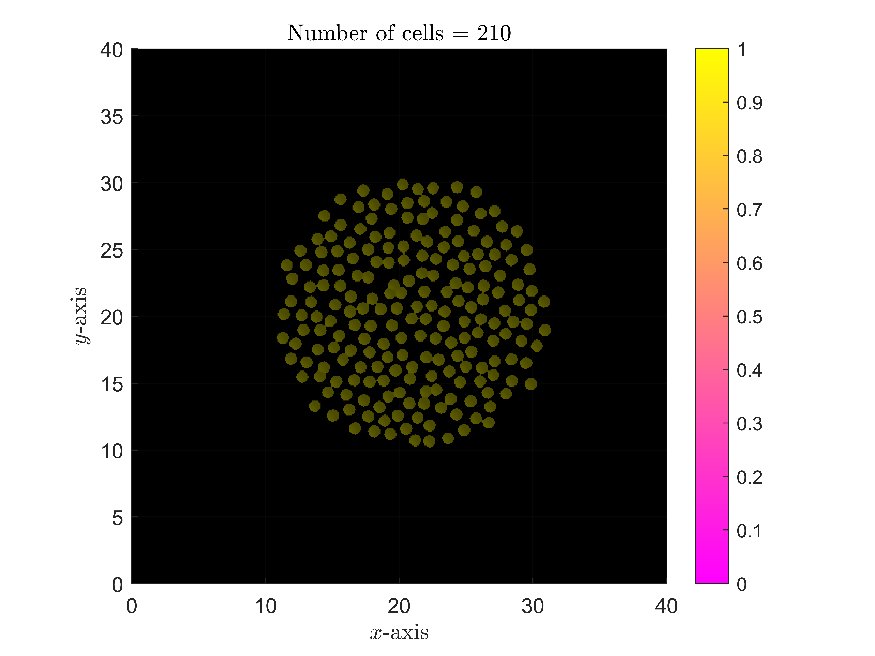
\includegraphics[width=1\textwidth]{chapter1/figures/ColonySimulationDemo_N_210.pdf}
\caption{The same colony at 210 cells}
\label{fig:ColonySimulationN210}
\end{figure}
\filbreak

\section{Adding in a nutrient field}


\begin{figure}[h]
\centering
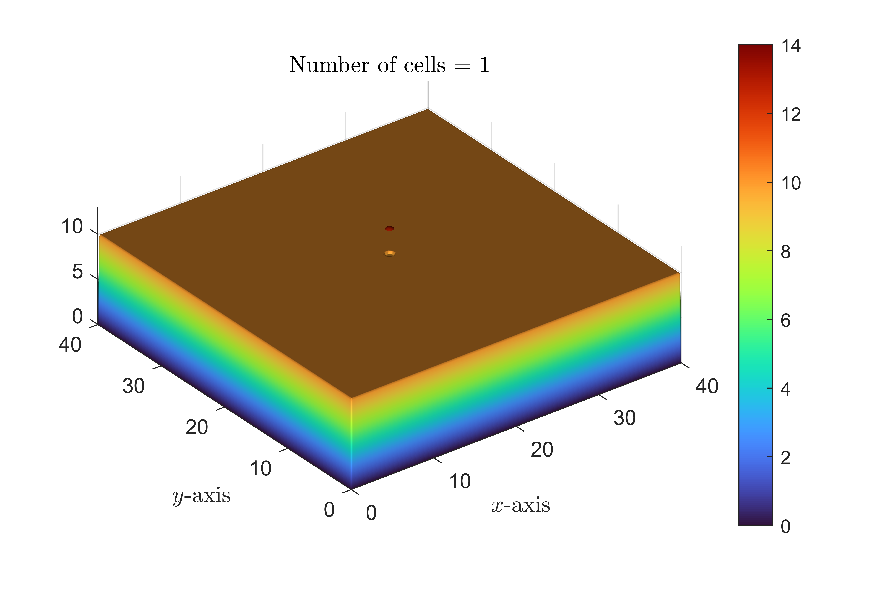
\includegraphics[width=1\textwidth]{chapter1/figures/ColonySimulationDemoNutrientField_N_1.pdf}
\caption{A starting configuration consisting of a cell with radius $1$ unit equals $3.5 \mu m$}
\label{fig:ColonySimulationStartingCellNutrientField}
\end{figure}
\filbreak


\begin{figure}[h]
\centering
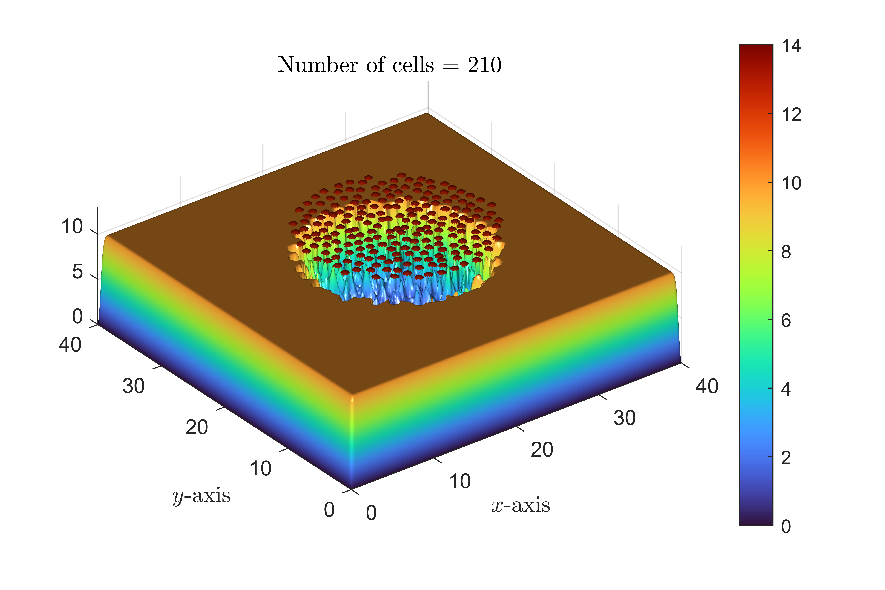
\includegraphics[width=1\textwidth]{chapter1/figures/ColonySimulationDemoNutrientField_N_210.pdf}
\caption{The same colony at 210 cells}
\label{fig:ColonySimulationNutrientFieldN210}
\end{figure}
\filbreak

\section{Simulating $N > 1000$ cells with a nutrient field}

Explain how I have used hash mapping to deal with cell collisions.

\begin{figure}[!htb] %Change this to [p] maybe ?
\centering
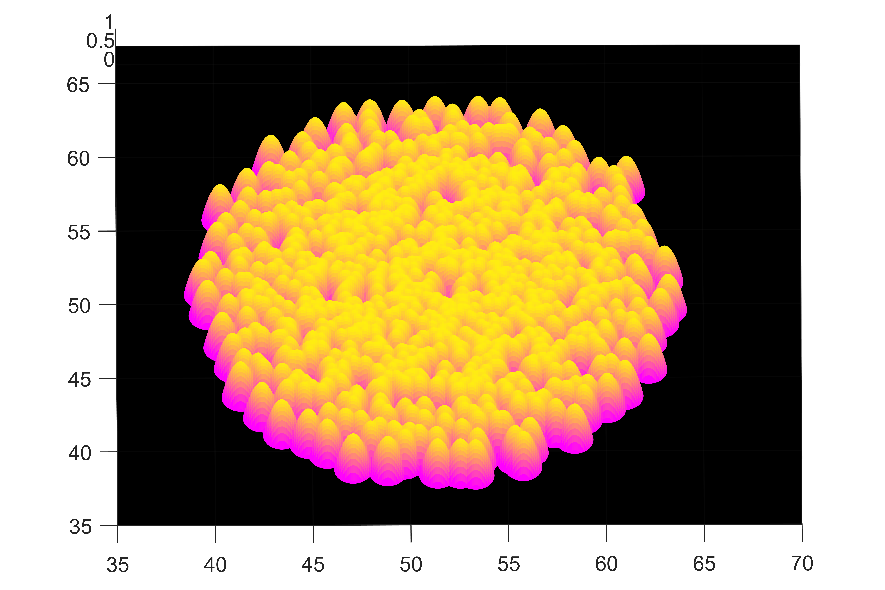
\includegraphics[width=1\textwidth]{chapter1/figures/ColonySimulationDemoNutrientField_N_1065.pdf}
\caption{A cell colony with 1065 cells }
\label{fig:ColonySimulationNutrientFieldN210}
\end{figure}
\filbreak



\section{Calculating the compactness metric}
A fully grown colony will in general not be perfectly circular in shape. In order to measure the roundness of the colony we use the metric used for roundness in image processing
\begin{equation}
    \Psi = \frac{P^2}{4 \pi A},
\end{equation}
where $\Psi \in [0,1]$ is $1$ for a perfect circle and can get to $0$ for highly non-round shapes, $A$ is the colony area, and $P$ is the colony perimeter. When the cells are undergoing mitosis, we are left with the issue of calculating roundness of the blended ``pill" shape geometry of two cells right before splitting. In affect, it will be necessary to calculate the length of 


\section{Collision Detection}

\begin{figure}
    \centering
    \begin{tikzpicture}


    
    \draw[->] (0,0) -- (3,0) node[right] {$x$};
    \draw[->] (0,0) -- (0,3) node[above] {$y$};
    \draw (0,0) circle (0.2);

    % Mass points and rod
    \draw[thick] (4,1) -- (8,2);

    % Mass m1
    \fill (4,1) circle (2pt) node[left] {$m_1$};
    % Mass m2
    \fill (8,2) circle (2pt) node[right] {$m_2$};

    % Center of mass
    \draw[fill=none] (6,1.5) circle (3pt);
    \node at (6.3,1) {$O_C$};

    % Distance markers
    \draw[<->] (4,1.2) -- (6,1.7) node[midway, above] {$d$};
    \draw[<->] (6,1.7) -- (8,2.2) node[midway, above] {$d$};

\end{tikzpicture}
    \caption{Shows a rod shaped backbone of an elliptical cell made from two masses $m_1 = m_2 = m$ connected by a massless rod of length $2d$}
    \label{fig:rod}
\end{figure}



\begin{figure}
    \centering
    \begin{tikzpicture}
    
    % Axes
    \draw[thick,->] (-1,0) -- (5,0) node[right] {$x$};
    \draw[thick,->] (0,-1) -- (0,5) node[above] {$y$};
    \draw[thick] (0,0) circle (0.15); % Rotational point

    % Rod
    \draw[thick]  (1,1) -- (4,3);
    
    % Points on the rod
    \fill (1,1) circle (0.07) node[below left] {1};
    \fill (4,3) circle (0.07) node[above right] {2};

    
    
    % Center of mass
    \draw[thick] (2.5,2) circle (0.15) node[right] {$O_C$};x

    %Center of action of force
    \fill (3.25,2.5) circle (0.07) node[above right] {P};

    % Forces
    \draw[->,thick] (3.25,2.5) -- ++(1,0.66667) node[above right] {$F_t$};
    \draw[->,thick] (3.25,2.5) -- ++(0,1.5) node[above] {$F$};
    \draw[->,thick] (3.25,2.5) -- ++(-0.8,1.2) node[left] {$F_n$};
    
    % Tangent and normal directions
    \draw[dashed] (4,3) -- ++(3,2) node[right] {$t$};
    \draw[dashed] (2.5,2) -- ++(-2,3) node[left] {$n$};

    %extra line for angle
    \draw[dashed] (1,1) -- ++(1.0,0)  node[right]{} ;

    % Angles
    %\draw[->] (1,1) ++(0.3,0.1) arc (0:30:0.3) %node[right] {$\theta_C$};
    %\draw[->] (2.5,2) ++(0.3,0.1) arc %(0:30:0.3) node[right] {$\theta_C$};

    \coordinate (A) at (1,1);
    \coordinate (B) at (1.5,1);
    \coordinate (C) at (1.416,1.2774);

    \draw pic["$\theta_C$",draw=green,<->,angle eccentricity=1.2,angle radius=1cm] {angle=B--A--C};

 
    \end{tikzpicture}
    \caption{Shows a rod shaped cell which is being impinged upon by a contact force $\vb{F}$ resolved into a tangential $F_t$ and normal component $F_n$.}
    \label{fig:rod_force}
\end{figure}

Referring to the supplied figures, we see that a force is $\vb{F}$ in Figure \ref{fig:rod_force} can be a representation of an applied force from another cell acting on the current cell. We set out to find forces on the two point mass that will produce equivalent force balance in the $(t,n)$ coordinate system.

We replace the force $\vb{F}$ with $\vb{F}_1$ and $\vb{F}_2$ acting on mass $1$ and $2$, respectively. From force balance
\begin{equation*}
 \vb{F}_1+  \vb{F}_2 = \vb{F}, 
\end{equation*}
and, from moment balance with anti-clockwise positive,
\begin{equation*}
 l_F F_n = d(F_{2,n} - F_{1,n}).
\end{equation*}
In our case, the impinging force will be from another cell, so we start by making the assumption that there is no tangential force, i.e. frictionless slipping. With this we can
derive simultaneous equations for $F_{1,n}$ and $F_{2,n}$ which have the solution
\begin{equation*}
    F_{1,n} =  \left( \frac{d-l_F}{2d} \right) F_n,
\end{equation*}

\begin{equation*}
    F_{2,n} =  \left( \frac{d+l_F}{2d} \right) F_n.
\end{equation*}
Assuming, once again, that $F_{1,t} = F_{2,t} = F_t = 0$ we can obtain the $(x,y)$ components by doing a coordinate transformation by the angle $-\theta_C = - \arctan{\left( y_2-y_1, x_2-x_1  \right)}$ where $(x_1,y_1)$ and $(x_2,y_2)$ are the mass positions, respectively. So, we have that the components of the force are given by 
\begin{equation*}
    \begin{bmatrix}
    F_{1,x} \\
    F_{1,y} 
    \end{bmatrix}
    =
    \begin{bmatrix}
    \cos{(-\theta_C)} & -\sin{(-\theta_C)}\\
    \sin{(-\theta_C)} & \cos{(-\theta_C)} 
    \end{bmatrix}
    \begin{bmatrix}
    -F_{1,n} \\
    0 
    \end{bmatrix}
    =
    \begin{bmatrix}
    \cos{\theta_C} & \sin{\theta_C}\\
    -\sin{\theta_C} & \cos{\theta_C} 
    \end{bmatrix}
    \begin{bmatrix}
    -\left( \frac{d-l_F}{2d} \right) F_n \\
    0 
    \end{bmatrix},   
\end{equation*}



\begin{equation*}
    \begin{bmatrix}
    F_{2,x} \\
    F_{2,y} 
    \end{bmatrix}
    =
    \begin{bmatrix}
    \cos{(-\theta_C)} & -\sin{(-\theta_C)}\\
    \sin{(-\theta_C)} & \cos{(-\theta_C)} 
    \end{bmatrix}
    \begin{bmatrix}
    F_{2,n} \\
    0 
    \end{bmatrix}
    =
    \begin{bmatrix}
    \cos{\theta_C} & \sin{\theta_C}\\
    -\sin{\theta_C} & \cos{\theta_C} 
    \end{bmatrix}
    \begin{bmatrix}
    \left( \frac{d+l_F}{2d} \right) F_n \\
    0 
    \end{bmatrix}.    
\end{equation*}
We solve this as
\begin{equation*}
  \vb{F}_1 =  - \left(\frac{d-l_F}{2d} \right)  F_n \cos{\theta_C} \hat{\vb{i}} + \left(\frac{d-l_F}{2d} \right)  F_n \sin{\theta_C} \hat{\vb{j}},
\end{equation*}

\begin{equation*}
  \vb{F}_2 =   \left(\frac{d+l_F}{2d} \right)  F_n \cos{\theta_C} \hat{\vb{i}} - \left(\frac{d+l_F}{2d} \right)  F_n \sin{\theta_C} \hat{\vb{j}},
\end{equation*}

\section{Approximate Bayesian Computation (ABC) for the inverse problem}
The traditional statement of Bayes' Theorem goes like
\begin{equation}
    P(A | B) = \frac{P(B|A) P(A)}{P(B)},
\end{equation}
where $A$ and $B$ are outcomes and the terms are given by
\begin{itemize}
    \item $P(A | B)$ is the posterior probability; the probability of $A$ given $B$,
    \item $P(B|A)$ is the conditional probability
    \item $P(A)$ is the prior probability; probability of observing event $A$
    \item $P(B)$ is the marginal probability; probability of observing event $B$
\end{itemize}








